%%%%%%%%%%%%%%%%%%%%%%%%%%%%%%%%

% Multiple Non-Collinear TF-map
% Alignment of Promoter Regions

%%%%%%%%%%%%%%%%%%%%%%%%%%%%%%%%

\chapter[Multiple Non-Collinear TF-map Alignment]
{\textbf{M}ultiple Non-Collinear\\ TF-map Alignment}\label{sec:mma}
\sectiongreen*{Summary}
\begin{center}
\begin{tabular}{c}
\fcolorbox{blue}{verylightgrey}{
\begin{minipage}[][4cm][c]{0.8\linewidth}
\sffamily
The generalization of the pairwise TF-map alignment is presented here. First, the 
formal definition of a multiple map alignment and how to compute the optimal score
is provided. Next, we use a progressive approach to build up a multiple alignment in
a stepwise manner. Then, we have studied how to break the non-collinearity property 
inherent to the alignments produced by dynamic programming techniques. Results
on biological data indicate that multiple TF-map alignments are able to locate regulatory
elements in several promoters that are not conserved at sequence level.
\end{minipage}}\\
\\[2ex]
\begin{minipage}[][4cm][c]{0.9\linewidth}
\minitoc
\end{minipage}
\end{tabular}
\end{center}
\newpage


\sectiongreen{The need for multiple TF-map alignment}\label{sec:motiv}

% A. (MULTIPLE) SEQUENCE ALIGNMENT IS IMPORTANT
\lettrine[lines=4,loversize=-0.1,lraise=0.1,lhang=.2]{S}{equence comparisons are 
one of the most important computational tools} in molecular biology. Sequences are 
good symbolic representations of biological molecules that encode relevant information 
about their structure, function and history. From the analysis of several related sequences, 
biologically significant facts can be inferred. For instance, genomic sequence comparisons
are performed in order to identificate genes or regulatory sites across
different genomes, as these functional elements tend to exhibit 
conservational patterns different from those observed in regions that are not 
functional.

%B. MULTIPLE SEQUENCE ALIGNMENT: PROGRESSIVE
In attempt to allow for multiple sequence comparisons, the basic dynamic
programming recurrences introduced in the 1970s to align efficiently two
sequences of $n$ symbols in $O(n^2)$ \citep{needleman:1970a,sellers:1974a},
can be naturally extended for $k$ sequences, with an exponential cost
$O(n^k)$ \citep{waterman:1976a}. As this cost is unaffordable in practice,
many heuristics have appeared to provide acceptable solutions with a minor cost.
The most popular of them is the hierarchical or clustering method
\citep{feng:1987a,thompson:1994a}. 

This procedure, also called progressive alignment, is a greedy algorithm
that runs in $O(k^2 n^2)$ time. In a first step, this method performs all
of the pairwise alignments to build an evolutionary tree. In a second step,
an initial alignment is constructed from the two closest sequences,
incorporating then the rest to the profile following the guide tree. Such a
procedure does not guarantee to find the optimal solution in mathematical
terms. However, the results are generally in good agreement with the
biological problem of aligning correctly bases of homologous functional
elements. See Chapter \ref{sec:algorithms} Section \ref{sec:msa} for a 
comprehensive review of this topic.

Progressive alignment has also commonly used in the genome-wide
alignment methods that perform rapid multiple genomic alignments to identify
conserved biological features between distant species. Basically, these
algorithms identify local similarities between two genomes that are then
used as anchors to align the interleaving regions \citep{delcher:1999a}.
The progressive technique is then combined with these genome pairwise
aligners to build up the multiple genome alignment \citep{brudno:2003a,bray:2004a}.

% C. THINGS ARE NOT ALWAYS CONSERVED AT THE SEQ LEVEL
These comparisons at the sequence level have limitations however. Although
similar sequences do tend to play similar biological functions, the opposite
is not necessarily true. Often similar functions are encoded in higher order
sequence elements that are not necessarily conserved at the sequence level.
As a result, similar functions are frequently encoded by diverse sequences
which are undetectable by conventional sequence alignment methods.

% D. PROMOTERS
Gene promoter regions are a good example. The information that governs the
RNA synthesis is mostly encoded in the gene promoter, a region normally $200$
to $2,000$ nucleotides long upstream of the transcription start site of the gene (TSS).
Transcription factors (TFs) bind to sequence specific motifs (the TF binding
sites, TFBSs) within the promoters. TFBSs are $5-8$ nucleotides long and one
promoter region contains on the order of $10$ to $50$ of them \citep{wray:2003a}.
Such motifs appear to be arranged in specific configurations that define the
temporal and spatial transcriptional pattern program of each gene. Genes
presenting similar expression patterns are assumed to share similar
configurations of TFBSs in their promoters. However, TFBSs associated to
the same TF are known to contain sequence substitutions, being in many
cases completely different. Promoter regions of genes with similar
expression pattern may not be similar at the sequence level, even though
they may be co-regulated.

% E. PREVIOUS WORK
In the previous chapter \citep{blanco:2006b}, we suggested the existence of 
regulatory information conserved between related promoters that could not be 
detected at the sequence level. Let $\Sigma_{TF}$ be the alphabet of TFs denoting
symbols. We initially defined the process of mapping a nucleotide sequence into a 
sequence in $\Sigma_{TF}$ (the TF-maps). Then, we developed an efficient algorithm 
to obtain the global pairwise alignment between two TF-maps \citep{blanco:2006b}. 
Finally, we showed the TF-map alignments were more accurate than conventional sequence 
alignment to distinguish pairwise gene co-expression in a collection of microarray 
results \citep{blanco:2006b}.

%%%%
% Figure 1: dummy mapping
%%%%
\begin{figure}[t!]
\begin{center}
\setlength{\fboxsep}{0pt}
\fbox{\incgraph{width=0.65\linewidth}{ps/dmapping}}
\mycaption{fig:dmapping}% label
          {TF-mapping in a simple example}% lof
          {TF-mapping in a simple example.}% caption header
          {}
\end{center}
\end{figure}

% F. PRESENT THIS PAPER 
In this chapter, we present an efficient implementation of
the multiple TF-map alignment based in the progressive alignment paradigm.
We have introduced some modifications in the pairwise global TF-map alignment
algorithm to align two clusters of TF-maps, eventually allowing non-collinear
arrangements of TFBSs in the results without additional cost. Most dynamic
programming global alignments rarely cope with the presence of rearrangements
observed in the DNA, being only partially identified by combining global and
local alignment strategies \citep{brudno:2004a,darling:2004a}. This problem is
particularly relevant in the case of the regulatory regions, where
non-collinear configurations of TFBSs are prone to be conserved
\citep{nix:2005a}. 

% G. STRUCTURE OF THE PAPER
The structure of the chapter is the following: first, we briefly reviewed the
concept of mapping functions and provide the formal definition of a multiple
TF-map alignment. Then, we introduce the main algorithm that performs the
progressive alignment of multiple TF-maps. Next, we detail the algorithm
to compute the optimal pairwise alignment of two clusters of maps. Later,
we define formally a non-collinear alignment, introducing some
modifications in the pairwise algorithm to allow the detection of these
cases. Finally, we systematically estimate the optimal parameters of the
alignment to distinguish promoters from other gene regions in a set of well
characterized human-rodent gene pairs and their corresponding orthologs in
chicken and zebrafish. These results are compared to those obtained by
conventional sequence alignment methods, showing the validness of our approach. 
Several particular examples are presented in which multiple TF-map alignments 
characterize conserved regulatory elements that are otherwise imperceptible 
in sequence-level comparisons.

%%%%
% Figure 2: dummy real
%%%%
\begin{figure}[t!]
\begin{center}
\setlength{\fboxsep}{0pt}
\begin{tabular}{|cc|}
\hline
A & \incgraph{width=0.65\linewidth,height=3cm}{ps/oneline}\\
B & \incgraph{width=0.65\linewidth}{ps/extended}\\
\hline
\end{tabular}
\mycaption{fig:rmapping}% label
          {TF-mapping of the human promoter NM\_015900}% lof
          {TF-mapping of the human promoter NM\_015900 ($500$ nucleotides).}% caption header
          {(A) Condensed representation of the TRANSFAC predictions.
           (B) The same set of predictions displayed in a non-overlapping format.}
\end{center}
\end{figure}

%%%%%%%%%%%%%%%%%%%%%%%%%%%%
%% Definitions            %%
%%
\sectiongreen{Basic definitions}

\subsectionblue{Mapping a promoter sequence into a TF-map}

Let $\Sigma_{DNA}$ be the alphabet of four nucleotides. Let $\Sigma_{TF}$ be 
the alphabet of TFs denoting symbols. In a previous work \citep{blanco:2006b}, 
we defined a mapping function as a procedure to translate a promoter region 
$S = s_1 s_2 \ldots s_k$ where each nucleotide $s_i \in \Sigma_{DNA}$, into a
sequence of TF-tuples $M = m_1 m_2 \ldots m_n$ where each TF-tuple 
$m_i=<m_i^f,m_i^{p1},m_i^{p2},m_i^s>$ denotes the match 
of a binding site for the TF $m_i^f \in \Sigma_{TF}$ occurring between the
position $m_i^{p1}$ and the position $m_i^{p2}$ over the sequence $S$
with score $m_i^s$. Different mapping functions can be used to obtain the 
translation from $S$ to $M$ such as a collection of weight matrices representing TFBSs
(JASPAR \citep{vlieghe:2006a}, PROMO \citep{farre:2003a} or TRANSFAC \citep{matys:2006a}). 
For each match over a given threshold, we register a new TF-tuple in $M$ defined 
by the label $(m_i^f)$ of the TF associated to the PWM, the positions 
$(m_i^{p1},m_i^{p2})$ and the score $(m_i^s)$ of the match (see Figure 
\ref{fig:dmapping}, for an example). Other mapping functions can used instead, such 
as pattern discovery programs that identify a set of unknown motifs conserved 
in several promoters (e.g. MEME \citep{bailey:1994a}).

Matches are annotated at a given location irrespective of their orientation 
in which they occur. This translation preserves the order of $S$ in $M$, that 
is if $i<j$ in $M$ then $(m_i^{p1} < m_j^{p1})$. Matches to different TFs may 
possibly occur at the same position, being false positives in most cases (see 
a real example in Figure \ref{fig:rmapping}). We refer to the resulting sequence 
of TF-tuples $M$ as a Transcription Factor Map, or simply a TF-map.

\subsectionblue{Multiple alignment of TF-maps} 
\index{alignment!mtfma@multiple TF-map alignments} \index{alignment!mmeta@multiple meta-alignments}
\index{TF-map alignments!mmetatf@multiple TF-map alignments}
\index{multiple TF-map alignments}
Let $M_1,M_2,\ldots,M_k$ be a set of TF-maps where each map is denoted
as $M_i = m_{i,1} m_{i,2} \ldots m_{i,|M_i|}$ and each TFBS is
denoted as $m_{i,j}^f \in \Sigma_{TF}$. Let $M_1^*,M_2^*,\ldots,M_k^*$
be the extended set of TF-maps where each map is denoted as $M_i^* =
m_{i,1}^* m_{i,2}^* \ldots m_{i,|M_i^*|}^*$, and each TFBS is denoted
as $m_{i,j}^{*f} \in \Sigma_{TF} \cup \{-\}$. The symbol $'-'$ indicates a
gap, which can be considered as a particular TF-tuple 
$<'-',\cdot,\cdot,\gamma>$ where the value $\cdot$ is a null value 
and $\gamma$ is the penalty for introducing a gap in a column of the alignment.

The alignment of $k$ maps $M_1,M_2,\ldots,M_k$ is then a correspondence $T$, maybe empty,
among the extended maps $M_1^*,M_2^*,\ldots,M_k^*$ such that:

\begin{enumerate}
\item
The extended maps have the same length.
\item 
If the gaps are removed from each $M_i^*$, we recover $M_i$.
\item
At least one element in a column is different from a gap.
\item
The elements that are aligned in a column correspond to the same TF.
\item
No overlap in the primary sequence is permitted between adjacent sites 
in the alignment.
\end{enumerate}

Note that the first three conditions define the classical multiple alignment 
of sequences. Last two conditions, however, introduce two new constrains that 
are related to the match state and the non-overlapping property, according to the 
notion of pairwise TF-map alignment provided in \citep{blanco:2006b}.


\subsectionblue{The score of a multiple alignment of TF-maps}

A multiple TF-map alignment --or simply, a multiple map alignment (MMA),
in contrast to a multiple sequence alignment (MSA)--
can be also represented as a rectangular array:

\begin{center}
\fcolorbox{white}{verylightgreen}{ 
\begin{minipage}[][][c]{0.95\linewidth}
\begin{equation}
T = \left(
\begin{array}{llll}
m_{1,1}^* & m_{1,2}^* & \ldots & m_{1,t}^*\\
m_{2,1}^* & m_{2,2}^* & \ldots & m_{2,t}^*\\
\ldots & & & \ldots\\
m_{k,1}^* & m_{k,2}^* & \ldots & m_{k,t}^*\\
\end{array}\right),
\end{equation}
\end{minipage}}
\end{center}

\noindent where each column $T(i)= (m_{1,i}^*,m_{2,i}^*,\ldots,m_{k,i}^*)$
is the multiple match among the TF-tuples in position $i$ from 
$M_1^*, M_2^* \ldots M_k^*$. Given the multiple alignment $T$, we compute the 
score $s(T)$ of the MMA as:

\begin{center}
\fcolorbox{white}{verylightgreen}{ 
\begin{minipage}[][][c]{0.95\linewidth}
\begin{equation}
s(T) = 
\begin{array}{ll}
  & \alpha \sum_{i=1}^t{\sum_{j=1}^k{m_{j,i}^{*s}}}\\
- & \lambda (g)\\
- & \mu \sum_{\forall i,i'}{f(m_{1,i}^{*p1}-m_{1,i'}^{*p1},m_{2,i}^{*p1} - m_{2,i'}^{*p1},\ldots,m_{k,i}^{*p1}-m_{k,i'}^{*p1})}
\end{array}
\label{eq:scorem}
\end{equation}
\end{minipage}}
\end{center}

\noindent where $\alpha,\lambda,\mu>0$, $g$ is the number of columns with only one
element different from a gap in the MMA (unaligned elements), and
$f$ is a function that measures the conservation of distance between the
sites of every map in two consecutive columns ($i,i'$) with more than one aligned element in the 
MMA. That is, the score of the alignment increases with the score of the aligned elements 
and the penalty of the gaps ($\alpha$), and decreases with the number of unaligned
elements ($\lambda$), and with the difference in the distance between adjacent aligned 
elements ($\mu$). See the previous chapter and \citet{blanco:2006b} for further details 
about the TF-map alignment parameters.

%%%%%%%%%%%%%%%%%%%%%%%%%%%%
%% The Algorithms         %%
%%
\sectiongreen{The algorithms}

There are many possible alignments between a group of TF-maps. The optimal
alignment is the one scoring the maximum among all possible alignments. In
a previous work \citep{blanco:2006b}, we implemented a dynamic programming
algorithm to obtain such an alignment efficiently for the case of two
TF-maps. The optimal multiple sequence alignment problem (and therefore
also the multiple alignment of maps) is, however, much more difficult, being 
formally a NP-complete problem \citep{wang:1994a}.

Here, we propose to adapt the popular progressive alignment strategy to
the TF-map alignment. The solutions obtained by this method are
not guaranteed to be optimal. However, multiple progressive alignments 
usually have an underlying biological explanation \citep{thompson:1994a}. 
We have also introduced some changes in the basic pairwise TF-map alignment 
algorithm developed in \citep{blanco:2006b}, in order to deal now with two 
clusters of MMAs instead of two single TF-maps. 

\subsectionblue{Progressive MMA algorithm}
\index{multiple TF-map alignments!progmmeta@progressive alignment}

Let $(G_1 \ldots G_k)$ be the initial list of $k$ TF-map groups,
where each group contains a single TF-map. Let $S$ be the similarity 
matrix where $S(G_i,G_j)$ denotes the similarity between the TF-map 
groups $G_i$ and $G_j$.

The progressive MMA algorithm shown in Figure \ref{fig:mmaalg} builds up a multiple TF-map
alignment in a stepwise manner. In a first step, all pairwise TF-map
alignments are performed. The initial multiple alignment is created 
with the two most similar ones. Both maps are substituted for a
new group that contains their alignment. The similarity between this
new cluster and the rest of the TF-maps is then estimated, updating
tha $S$ matrix (see Implementation).

In a second step, an iterative procedure selects at each round the pair
of clusters that are more similar from the pool of available groups.
These two groups are aligned and merged again into a new TF-map cluster,
estimating the similarity to the remaining ones. At the end of the
process, there is only one group that contains the progressive alignment
of the input TF-maps.

The cost of the progressive MMA can be expressed in terms of the number
of pairwise TF-map alignments that must be computed. Let $k$ be the number
of maps to be aligned and $n$ be the length of each map. The initial round
performs $O(k^2)$ pairwise alignments. Next, the progressive round performs
$O(k)$ alignments involving two groups. Let $P(n)$ be the cost of each
pairwise operation, then the cost of the progressive alignment algorithm
is $O(k^2 \cdot P(n))$. The expected value of $P(n)$ is calculated in the
next section.


%%%%
% Figure 4: Progressive Multiple Map Alignment
%%%%
\begin{figure}[t!]
\begin{center}
\scalebox{1}{
\fcolorbox{white}{verylightgreen}{
\begin{minipage}[][][c]{\linewidth}
\begin{algorithmic}[5]
\REQUIRE $G$: list of TF-map groups $(G_1 \ldots G_k)$
\STATE
\STATE \COMMENT{ Initial Step: pairwise alignment all Vs all }
\STATE maxSim $\leftarrow -\infty $
\FOR{$i=1$ to $k$}
\FOR{$j=i+1$ to $k$}
\STATE $S(G_i,G_j) \leftarrow$ ComputePairwiseSimilarity$(G_i,G_j)$;
\STATE \COMMENT{Select the pair with maximum similarity}
\STATE maxSim $\leftarrow$ max(maxSim,$S(G_i,G_j)$);
\ENDFOR
\ENDFOR
\STATE \COMMENT{Create a new group: estimate the similarity to others}
\STATE $G_{iSim-jSim} \leftarrow$ MergeGroups$(G_{iSim},G_{jSim})$;
\STATE
\STATE \COMMENT{ Progressive Step: cluster the two most similar groups }
\WHILE{$|G| > 1$}
\STATE maxSim $\leftarrow -\infty $
\FOR{$i=1$ to $|G|$}
\FOR{$j=i+1$ to $|G|$}
\STATE \COMMENT{Select the pair with maximum similarity}
\STATE maxSim $\leftarrow$ max(maxSim,$S(G_i,G_j)$);
\ENDFOR
\ENDFOR
\STATE \COMMENT{Create a new group: estimate the similarity to others}
\STATE $G_{iSim-jSim} \leftarrow$ MergeGroups$(G_{iSim},G_{jSim})$;
\ENDWHILE
\end{algorithmic}
\end{minipage}}}
\mycaption{fig:mmaalg}% label
          {Progressive multiple map alignment algorithm}% lof
          {Progressive multiple map alignment algorithm.}% caption header
          {}
\end{center}
\end{figure}


\subsubsectionblue{Implementation}

In the progressive MMA algorithm shown in Figure \ref{fig:mmaalg}, the variable \emph{maxSim}
saves the maximum score so far computed at each round. The group
identifiers of such a score can easily be retrieved using a supplementary
pair of variables \emph{iSim, jSim}.

The pairwise TF-map alignment algorithm called
\emph{ComputePairwiseSimilarity} \citep{blanco:2006b} has been slightly
modified to accomodate the alignment of two TF-maps groups, as explained in
the next section. The optimal pairwise alignments between the input TF-maps
in the initial round are saved, as they could be required during the
iterative procedure.

Once a new TF-map group is created from the two most similar ones, their
binding sites must be merged (function \emph{MergeGroups}). The order of
the TFBSs in the new group must take into account the position of the
binding sites in their primary promoter sequences. In the approach here, we
do not create a profile of each MMA. Instead, all of the TFBSs of each group
are always available for subsequent TF-map alignments.

The alignments between this new TF-map group and each one of the
rest of the groups are not explicitly computed. The similarity among
them is instead estimated with the WPGMA method (Weighted Pair Group Method 
with Arithmetic Mean) according to the previous similarity between the 
groups $G_{iSim}$ and $G_{jSim}$ to the others. If an alignment between 
two groups whose similarity was estimated before is identified as the most similar 
during the progressive step, the MMA must be explicitly computed before merging 
both TF-map groups.

%%%%
% Figure 5: DP matrix
%%%%
\begin{figure}[t!]
\begin{center}
\setlength{\fboxsep}{0pt}
\fbox{\incgraph{width=0.75\linewidth}{ps/mmads}}
\mycaption{fig:mmads}% label
          {MMA algorithm: data structures and matrix}% lof
          {MMA algorithm: data structures and similarity matrix.}% caption header
          {}
\end{center}
\end{figure}


\subsectionblue{The alignment of two clusters of MMAs}
\index{multiple TF-map alignments!clusmmeta@alignment of two clusters}

Let $G_x = m_{x,1} m_{x,2} \ldots m_{x,|G_x|}$ and 
$G_y = m_{y,1} m_{y,2} \ldots m_{y,|G_y|}$ be the two most similar groups of 
TF-maps in the current round of the progressive alignment. Let $S$ be the scoring 
dynamic programming matrix where $S(i,j) = S(m_{x,i},m_{y,j})$ denotes the similarity 
of the best TF-map alignment of the groups $G_x=m_{x,1} \ldots m_{x,i}$ and 
$G_y=m_{y,1} \ldots m_{y,j}$, according to the scoring function in Equation \ref{eq:scorem}.
The \emph{ComputePairwiseSimilarity} algorithm explained here is a generalization of 
that developed in \citep{blanco:2006b} to align two TF-maps that computes the optimal 
pairwise TF-map alignment between $G_x$ and $G_y$.

This algorithm basically searches the the maps of 
both groups to find matches between one site in one group and one site in the other. 
Once a new match is identified, the previous matches must be evaluated
in order to construct the optimal alignment ending at this one (see Figure \ref{fig:mmads}).
Because this class of scoring matrices are highly sparse, 
we register the coordinates in $S$ of the matches computed previously. 
Thus, to compute the optimal score at the cell $S(i,j)$, only the 
non-empty cells in $S$ that are visible for the current match need to be accessed. 
In addition, we maintain the list sorted by optimal score, so that the cell scoring the 
maximum value is at the beginning of the list and, in most cases, only a few nodes will
need to be accessed before a critical node is reached beyond which the
optimal score can not be improved \citep{blanco:2006b}.

The number of computations $P(n)$ in this algorithm is very similar
to that obtained in the conventional pairwise TF-map alignment algorithm
\citep{blanco:2006b}. The exact complexity of this algorithm is
difficult to be studied --depending mostly on the size of the input maps
and the sparsity of the resulting marix $S$. An expected time cost
analysis reveals that the cost function can be explained in terms of (a)
a first quadratic term derived from the obligatory comparison between all
of the TFBSs of both maps to detect the match cells and (b) a second
quadratic term necessary to search for each match the best adjacent previous
pair in the optimal TF-map alignment. In \citep{blanco:2006b}, we studied
the contribution of using a list of non-empty cells in $S$ that
reduces the second component to an expected cost of $O(p \cdot n^2)$, where $p$ is
the percentage of the matrix that is occupied. This value was estimated to be 
below 5\% of occupancy for the pairwise TF-map promoter comparisons.


%%%%
% Figure 6: ComputeSimilarity$(G_i,G_j)$
%%%%
\begin{figure}[t!]
\begin{center}
\scalebox{1}{
\fcolorbox{white}{verylightgreen}{
\begin{minipage}[][][c]{\linewidth}
\begin{algorithmic}[5]
\REQUIRE $G_x,G_y$: TF-map groups, $L$: list of $<$abscissa,ordinate$>$, $L = \emptyset$ 
\STATE \COMMENT{Calculating the element $i,j$ in $S$}
\FOR{$i=0$ to $|G_x|-1$}
\FOR{$j=0$ to $|G_y|-1$}
\IF{factor$(m_{x,i})$ = factor$(m_{y,j})$}
\STATE $S(i,j) \leftarrow$ ComputeInitialSimilarity($m_{x,i},m_{y,j}$);
\STATE $x \leftarrow \alpha$ (score$(m_i)$ + score$(m_j)$);
\STATE \COMMENT{Searching the best previous match in $L$}
\STATE $p \leftarrow$ first($L$);
\STATE $i' \leftarrow$ abscissa($p$);
\STATE $j' \leftarrow$ ordinate($p$);
\WHILE{end($L$) = FALSE and $S(i',j') + x > S(i,j)$}
\STATE \COMMENT{Compute the $\mu$ value and check overlap}
\STATE $(D_1,D_2,$overlap) $\leftarrow$ ComputeOverlap($i,i,j,j',G_x,G_y$);
\IF{overlap $=$ FALSE}
\STATE $y \leftarrow \lambda$ (ComputeLambda$(i,i,j,j')$);
\STATE $z \leftarrow \mu (|D_1 - D_2|)$; 
\STATE maxSim $\leftarrow S(i',j') + x - y - z$;
\IF{maxSim $> S(i,j)$}
\STATE $S(i,j) \leftarrow$ maxSim; 
\ENDIF
\ENDIF
\STATE $p \leftarrow$ next($L$);
\STATE $i' \leftarrow$ abscissa($p$);
\STATE $j' \leftarrow$ ordinate($p$);
\ENDWHILE
\STATE $n \leftarrow$ CreateNewNode($i,j$);
\STATE InsertNode($n,L$);
\ENDIF
\ENDFOR
\ENDFOR
\end{algorithmic}
\end{minipage}}}
\mycaption{fig:clusteralg}% label
          {Pairwise alignment of two clusters of TF-maps}% lof
          {Pairwise alignment of two clusters of TF-maps.}% caption header
          {}
\end{center}
\end{figure}

\subsubsectionblue{Implementation}

In the pseudocode in Figure \ref{fig:clusteralg}, the groups $G_x$ and $G_y$ are represented as
two arrays of sites sorted by the position in their promoters, where each 
site corresponds to an input TFBS. The multiple TF-map alignment of a cluster 
is internally encoded with pointers among the sites that form each match. 
Gaps here are not explicitly represented. 

Each site $m_{x,i}$ is a structure as described above with the functions 
\emph{factor, pos1, pos2 and score} returning the values of the corresponding fields. 
The variable \emph{maxSim} stores the optimal score so far computed.
The sites in the optimal TF-map alignment can be easily retrieved using
a supplementary structure \emph{path(i,j)} that points to the previous
cell in the optimal path leading to cell $S(i,j)$. In addition, the 
function \emph{ComputeInitialSimilarity} calculates for each match 
$S(i,j)$ the initial score of a hypothetical alignment that includes only 
the sites $m_{x,i}$ and $m_{y,j}$.

Once the match between two sites $m_{x,i}$ and $m_{y,j}$ has been identified,
the best previous match between two other sites $m_{x,i'}$ and $m_{y,j'}$ is
used to construct the new alignment (see the matches $A$ and $B$ in Figure
\ref{fig:mmads}). The list $L$ is used to locate the non empty positions in $S$.
Each node of the list $L$ is represented as structures $p$ and $n$ 
with the functions \emph{abscissa} and \emph{ordinate} returning the 
corresponding coordinates in $S$ of each previous match. 

The score of the new match between $m_{x,i}$ and $m_{y,j}$ is the sum of 
the scores of the columns in which both elements were aligned in their respective 
MMAs. Unaligned sites are scored with the gap penalty $\gamma$.
The function \emph{ComputeLambda} counts the number of sites
in each group that are not included in the alignment, taking into
account the size of each group. The function \emph{ComputeOverlap} calculates the 
average distances $D1$ and $D2$ between any pair of consecutive matches in the maps of 
both groups, verifying the absence of physical overlap in their promoters.
The function $|D1-D2|$ scores the conservation of distance between the sites of every 
map in two consecutive columns in the MMA (function $f$, see Equation \ref{eq:scorem}).


\sectiongreen{Non-colinear TF-map alignments}
\index{multiple TF-map alignments!noncolmmeta@non-collinear alignments}
\index{TF-map alignments!noncolmeta@non-collinear alignments}

The existence of regulatory elements that are conserved in different order
between related promoter regions is documented, specially in enhancers
\citep{nix:2005a}. Even at the sequence level, the identification of these
DNA rearrangements is very difficult.
We have here introduced some subtle changes in the pairwise TF-map 
alignment algorithm shown before to deal with non-collinear alignments.
The aligned TFBSs in such MMAs are therefore not necessarily located in
the same relative order in every map.

%%%%
% Figure 8: NON-COL alns
%%%%
\begin{figure}[t!]
\begin{center}
\setlength{\fboxsep}{0pt}
\fbox{\incgraph{width=0.65\linewidth}{ps/noncol}}
\mycaption{fig:noncol}% label
          {Two examples of non-collinear MMAs}% lof
          {Two examples of non-collinear MMAs.}% caption header
          {(Left) A pairwise non-collinear TF-map alignment. (Right) A non-collinear MMA.}
\end{center}
\end{figure}

\subsectionblue{Definition}

Let T be an alignment between two TF-maps $M_1$ and $M_2$ formally defined as
a correspondence $T=\{(m_{1,I_1},m_{2,J_1}), \ldots, (m_{1,I_t},m_{2,J_t}) \}$.
Let $(m_{1,i},m_{2,j})$ and $(m_{1,k},m_{2,l})$ two matches in $T$
,not necessarily contigous, with $i<k$. Then, we define the collinearity or
non-collinearity of $T$ in terms of the ordering between $j$ and $l$,
for all the match pairs of $T$ as:

\begin{enumerate}
\item
If $j<l$ then $T$ is a collinear alignment
\item
If $j>l$ then $T$ is a non-collinear alignment
(see example shown in Figure \ref{fig:noncol} (Left).
\end{enumerate}

The generalization of this definition for $k>2$ TF-maps is immediate
(see the example of a non-collinear MMA for $k=3$ TF-maps in Figure
\ref{fig:noncol} (Right).

%%%%
% Figure 9: NON-COL matrix
%%%%
\begin{figure}[t!]
\begin{center}
\setlength{\fboxsep}{0pt}
\fbox{\incgraph{width=0.65\linewidth}{ps/areas}}
\mycaption{fig:areas}% label
          {Diagonal filling of the alignment matrix}% lof
          {Diagonal filling of the alignment matrix.}% caption header
          {}
\end{center}
\end{figure}


\subsectionblue{The algorithm}

The non-collinear matches shown in Figure \ref{fig:noncol} can not be detected
in the basic pairwise TF-map alignment algorithm. Let $A$ and $B$ be two
TF-maps in which two matches could form a non collinear alignment
(represented as a circle and a square in Figure \ref{fig:areas}). The
normal implementation fills in the matrix row by row, from top to bottom
(or column by column, from left to right).
According to this, when the first match is being processed (red square),
the second one (red circle) is not still available (green area). On the
contrary, when the second match is processed, the first one is not
accessible as the basic algorithm only allows the search for best previous
aligned elements in the list of computed values that are in the area
delimited by the current match.

To overcome such a limitation, we propose to compute the optimal values of the
matrix $S$ following a different order, to allow the visibility of one of
these elements (circle) by the other (square). For instance, the top-bottom
diagonal filling of the matrix depicted in Figure \ref{fig:areas} may process
in first position the element that was not visible before (circle) for the
other element (square) that will computed later in the next diagonal (square).
While this strategy still produces the same aligments obtained with the
ordinary implementation, non-collinear alignments produced by new
combinations of matches can also be formed.

\subsubsectionblue{Adjusting the non-collinearity}
Non-collinear conservation of regulatory elements is documented
in very specific cases \citep{nix:2005a}. Most upstream promoter
regions, however, are constituted of collinear arrangements of TFBSs.
Because of the poor specificity of the collections of PWMs \citep{schones:2005a}, 
many non-collinear alignments produced with the algorithm described above 
are simply artifacts. 

Thus, we have designed a simple mechanism to adjust the frequency of
non-collinear aligned sites in the output. As the function \emph{ComputeOverlap}
in the algorithm above needed to be redefined in order to detect
non-overlap between non-collinear matches as well, we have introduced
an additional parameter $c$ to weight those alignments involving
non-colinearity.

The following example is graphically presented in Figure \ref{fig:graph} (Left).
Let $A$ and $B$ be two TF-maps in which a previous match has been 
identified (represented as a circle). Then, a second match between 
an element in $A$ and another in $B$ is being processed (the squares).
The dotted lines indicate that such a site in $B$ can be located either 
on the left or on the right of the circle site in the same map. In the
first case, a non-collinear alignment is produced; in the second case,
a normal collinear alignment is constructed. 

%FORMULA
The algorithm to align two clusters of TF-maps must be slightly modified 
to accomodate the non-collinearity parameter $c$ (the case in which the 
non-collinear match occurs in $A$ can be similarly defined):

\begin{center}
\fcolorbox{white}{verylightgreen}{ 
\begin{minipage}[][][c]{0.5\linewidth}
\begin{equation}
z = 
\left\{
\begin{array}{ll}
\mbox{if} ~~ (D_2 < 0)& \rightarrow \mu |D_1 - c \cdot D_2|, c \geq 1\\[2ex]
\mbox{if} ~~ (D_2 \geq 0)& \rightarrow \mu |D_1 - D_2|
\end{array}\right..
\label{eqnoncol}
\end{equation}
\end{minipage}}
\end{center}

The optimal positional conservation between both matches occurs when $d_1 = d_2$.
However, the parameter $c$ is used into the $\mu$ penalty to punish only those
matches that do not respect the collinearity of the current alignment (the square
site is on the left of the circle site in $B$, see Figure \ref{fig:graph}). 

Informally, if $c=1$ then both collinear and non-colinear matches are indistinctly 
combined into the resulting MMA. High values of $c$, however, produce a higher amount 
of collinear matches into the results. In order to establish formally the behaviour of 
this parameter, we have count the number of non-collinear matches in the TF-map alignment
of the human and mouse promoters ($500$ nucleotides) of the MMP13 gene (\refseq{} entries 
NM\_002427 and NM\_008607). In Figure \ref{fig:graph}, there is a clear correspondence between the 
amount of inversions in the MMA and the value of $c$. No inversions are produced for large 
values of $c$.

Identification of non-collinear configurations of TFBSs in regulatory regions
is poorly known. We recommend, therefore, to use this option very carefully. In
addition, we also suggest the use of a small set of matrices to perform the
mapping, which can reduce the number of artifacts in the resulting
non-collinear MMA.

%%%%
% Figure 11: NON-COL parameter
%%%%
\begin{figure}[t!]
\begin{center}
\setlength{\fboxsep}{0pt}
\fbox{\incgraph{width=0.75\linewidth}{ps/ncparam}}
\mycaption{fig:graph}% label
          {The non-collinearity parameter}% lof
          {The non-collinearity parameter.}% caption header
          {}
\end{center}
\end{figure}

%%%%%%%%%%%%%%%%%%%%%%%%%%%%
%% Results                %%
%%
\sectiongreen{Biological results}

The optimal MMA of a set of TF-maps is obviously dependant on the
values of the $\alpha, \lambda, \mu, \gamma$ and $c$ parameters. In addition,
the optimal parameter configuration is likely to depend on the particular
problem to be addressed (orthologous genes or co-regulated genes in microarray
experiments), and the particular protocol to map the TFBSs on the sequences.

Results in the previous chapter \citep{blanco:2006b}, indicated that TF-maps
alignments are able to characterize promoter regions of co-regulated genes
in absence of sequence similarity. Thus, TF-map alignments were shown to
detect high-order regulatory signals conserved in a collection of
related promoters that were undetectable for current sequence alignment
methods. It is important to mention that two different TFBSs can
be aligned if they correspond to the same TF, irrespectively of their 
sequence motifs.

%%%%
% Figure 12: 
%%%%
\begin{figure}[t!]
\begin{center}
\setlength{\fboxsep}{0pt}
\fbox{\incgraph{width=0.65\linewidth}{ps/testregions}}
\mycaption{fig:testregionsM}% label
          {Distinguishing promoters from other genomic regions}% lof
          {Distinguishing promoters from other genomic regions.}% caption header
          {}
\end{center}
\end{figure}

Here we have conducted a similar systematic training over an extended set
of orthologous promoters for obtaining the optima configuration. In order
to verify the ability of MMA to identify regulatory elements that are
rarely detected in conventional comparisons, we have compared the results
to those obtained by global sequence alignment methods. In addition, we
have focused on three specific examples to show the abilities of MMA in the
characterization of co-regulated gene promoters. In all of the cases, we have 
only constructed collinear map alignments as non-collinear regulatory 
rearrangements have not been reported on them.

\subsectionblue{Multiple TF-map training}
\index{multiple TF-map alignments!trainingmmeta@training}

For the pairwise TF-map alignment, we estimated the optimal parameters
in a set of experimentally characterized human and rodent gene promoters
\citep{blanco:2006b}. Here we have extended such a dataset by searching
the corresponding orthologs in chicken and zebrafish as well. Using the
\refseq{} \citep{pruitt:2005a} gene set as mapped into the UCSC genome browser,
we have correctly identified the ortholog in both species, if available.
We refer to the resulting set of human-mouse-chicken-zebrafish homologous 
genes as the \textsc{HRCZ set}. This dataset contains $18$
human-rodent-chicken-zebrafish orthologs, $7$ human-rodent-chicken orthologs,
$4$ human-rodent-zebrafish orthologs, and $7$ human-rodent orthologs.

The lack of available collections of experimentally verified TFBSs is
an important limitation for the evaluation and the training of phylogenetic 
footprinting systems. Despite several databases of annotations and promoter
sequences have recently appeared \citep{blanco:2006a,xuan:2005a}, there 
is not a minimum amount of regulatory information conserved among species 
other than human and mouse to train the MMA on them.

%%%%%%%%%%%%%%%
%%% TABLE 1
%%%%%%%%%%%%%%%
\begin{table}[t!]
\begin{center}
\begin{minipage}{0.95\linewidth}\setlength{\parindent}{0pt}
\begin{center}
\scalebox{0.75}{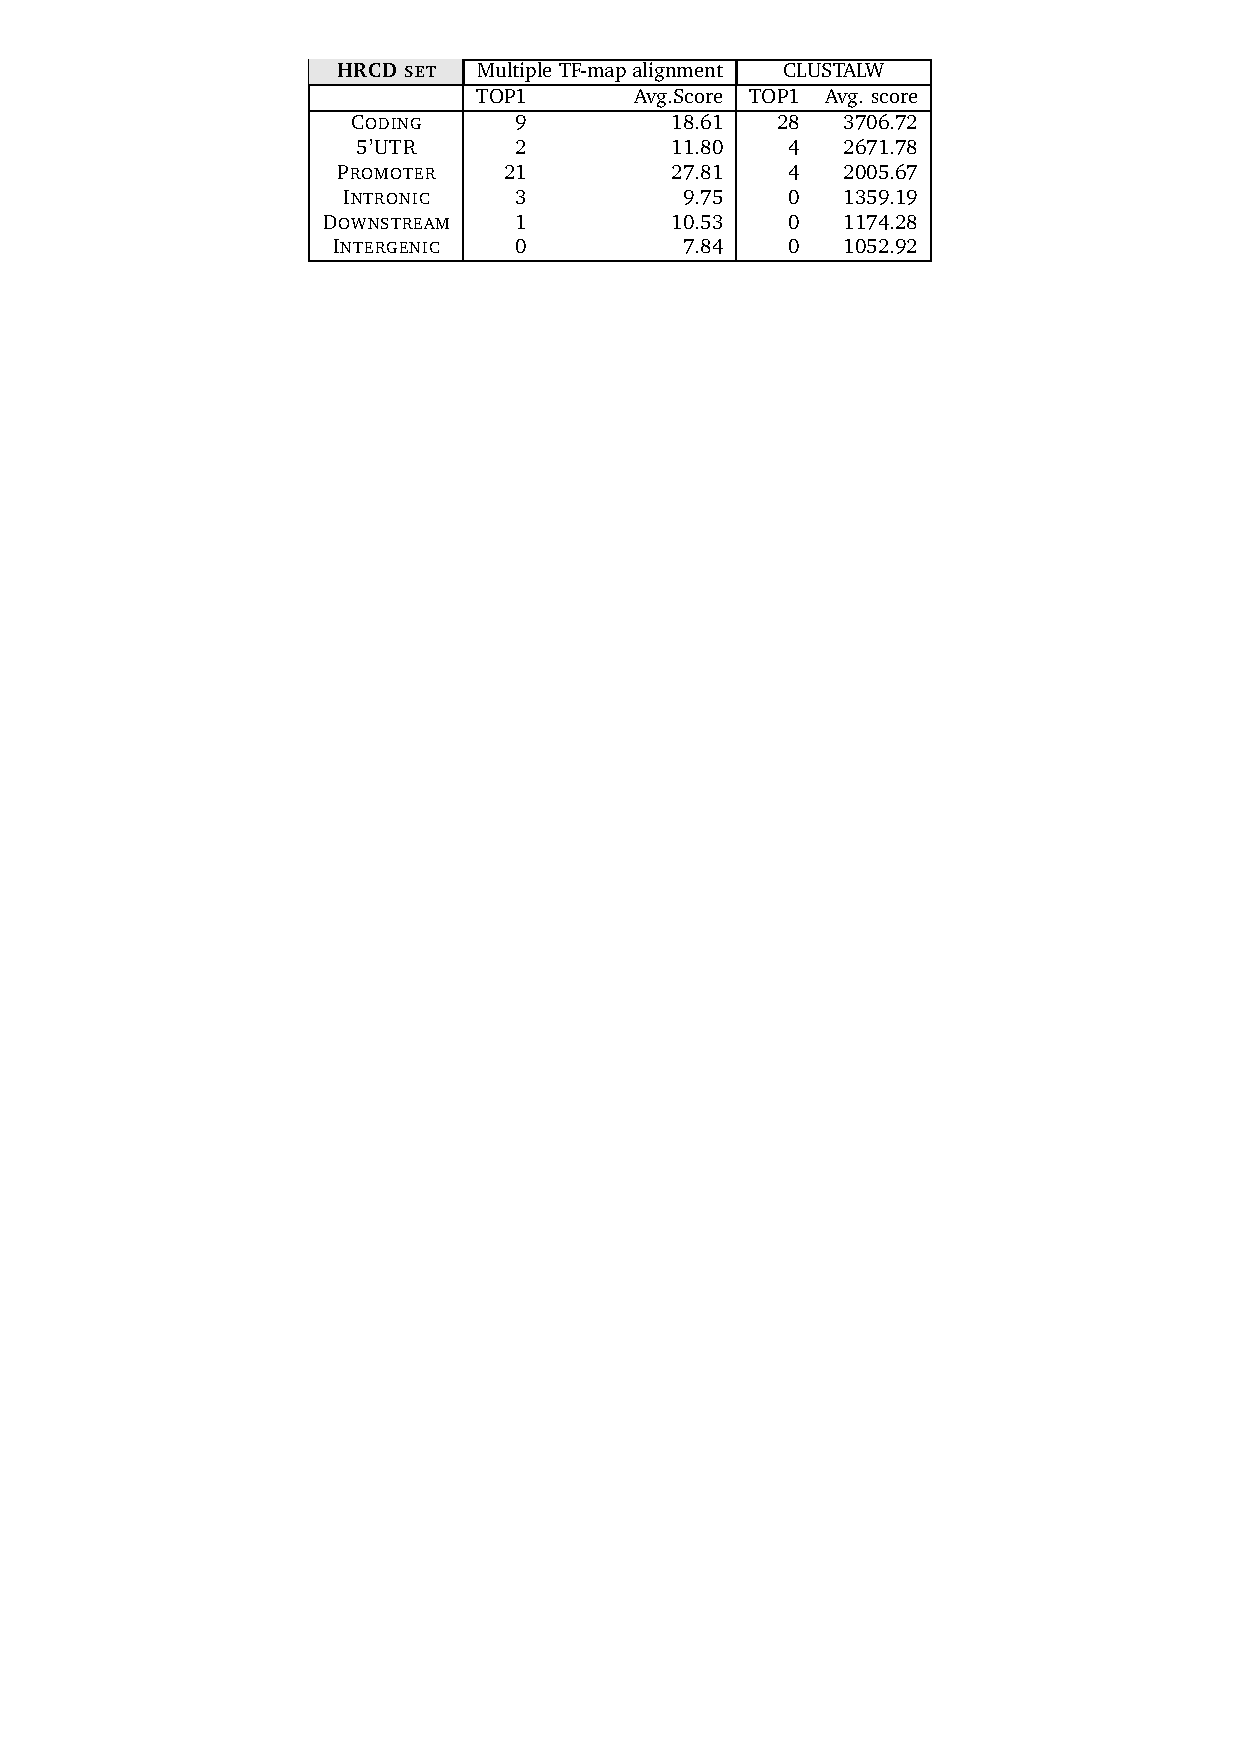
\includegraphics[bb=141 715 449 817,clip]{tables/testregionsM}}
\end{center}
\end{minipage}
\mycaption{tab:testregionsM}% label
          {Results when distinguishing promoters with MMAs}% lof
          {Results when distinguishing promoters with MMAs.}% caption header
          {}
\end{center}
\end{table}

Thus, we can not repeat the training procedure used in \citep{blanco:2006b}
to evaluate the ability of MMA to detect conserved regulatory elements at
larger evolutionary distances --at which the degree of conservation may
be negligible. However, we can use another method, also presented in
\citep{blanco:2006b}, to show that MMAs are much more informative than
primary multiple sequence alignments.

We first have mapped the TFBSs occurrences in the promoter sequences
using the collection of 50 most informatives matrices in \db{JASPAR} 1.0
\citep{sandelin:2004a}, to which we refer as \db{JASPAR$_{TOP50}$} \citep{blanco:2006b}.

Then, we have compared the MMAs obtained in the $200$ nucleotides of the
promoter region of the 36 gene pairs from the \textsc{HRCZ set}, with the
MMAs obtained in fragments of $200$ nucleotides from intergenic ($2,000$
nucleotides upstream of the TSS), 5'UTR (downstream of the TSS), coding
(downstream of the translation start site and considering only coding DNA),
intronic (downstream of the first intron junction), and downstream
(downstream of the transcription termination site) sequences (see
Figure \ref{fig:testregionsM} for a graphical representation of the test).
We have computed the average score of the MMA on each one of the genomic
regions and have identified, for each orthologous set, the genome regions
in which the alignment produces the highest score. We have performed the
same exercise using global pairwise sequence alignments (obtained with
CLUSTALW, \citep{thompson:1994a}).

We have repeated this test using different combinations of parameters.
Systematically, the parameters $\alpha, \lambda$ and $\mu$ were allowed
to independently take values between $0.0$ and $1.0$, in incremental steps
of $0.1$. At the same time, the parameter $\gamma$ (gap penalty) was
tested between $0$ and $-10$. The optimal parameter configuration is 
considered to be that set of parameter values that better discriminate 
between promoters and the rest of genomic regions.

Results appear in Table \ref{tab:testregionsM}. As expected, nucleotide sequence
alignments score the highest in the coding regions (in $28$ out of $36$
cases), followed by the alignments in the 5$^\prime$ UTR regions ($4$
out of $36$) and in the promoters ($4$ out of $36$). The scores of the
sequence alignments show that promoter regions are less conserved than
coding regions, and 5'UTRs. Despite this, the optimal MMA configuration
in the collinear configuration $(\alpha=1,\lambda=0.1,\mu=0.1,\gamma=-2)$
scores the highest in the promoter regions (in $21$ out of $36$, see Table \ref{tab:testregionsM}).
In addition, the average score of map alignments is notably higher than that of
the coding regions. Only in $9$ out of $36$ cases the TF-map alignments score
the highest in coding regions. Interestingly, while intron sequences in the
human-mouse-chicken-zebrafish orthologs are much less conserved than 5'UTRs,
MMAs score the highest in intronic regions in $3$ cases whereas they only
score the best in 5'UTRs in $2$ cases. This is consistent with the fact that
first introns are known to often contain regulatory motifs.

%Shuffle test
Finally, we have also performed a complementary test to measure the 
specificity of the TF-map alignments. As a negative control, we have shuffled 
the orthologous associations in the \textsc{HRCZ set} to construct a pool of 
unrelated human-mouse-chicken-zebrafish $36$ gene entries. Then, the 
corresponding multiple TF-map alignments of these non-orthologous paired
promoters were obtained using the parameters previously optimized.
The TF-map alignments of the unrelated promoters of each entry were 
significantly worse with an average score more than 50\% smaller than 
TF-map alignments that involved ``bona fide'' orthologous promoters. 
For instance, the average score of the TF-map alignments among orthologous 
promoters when using the \db{JASPAR$_{TOP50}$} collection was $27.81$. In contrast, 
the score of the TF-map alignments between non-related promoters was $12.51$. 
The sites in the alignments involving non-orthologous gene promoters may 
hypothetically correspond to general regulatory elements present 
in most core promoters. An alternative, more probable, hypothesis is that they
reflect the poor specificity of most PWMs representing TFBSs.

\subsectionblue{Promoter characterization}

We have selected three examples to show the ability of MMAs to characterize
promoter regions in the absence of sequence conservation. In the three cases, 
we have compared the multiple TF-map aligment against the corresponding multiple 
sequence alignment produced by CLUSTALW, as in the section above. 

All of the cases are graphically represented as pictures in which the
input TF-maps are displayed on the upper part of the picture and the
resulting MMAs are displayed on the lower part of the picture, using the
\prog{gff2ps} program \citep{abril:2000a}.

%%%%
% Figure 13: 
%%%%
\begin{figure}[t!]
\begin{center}
\setlength{\fboxsep}{0pt}
%\fbox{
\incgraph{width=0.9\linewidth}{ps/a00}%}
\mycaption{fig:A00s}% label
          {Multiple promoter characterization}% lof
          {Multiple promoter characterization.}% caption header
          {(Top) \db{JASPAR} predictions and the MMA among the \emph{Actin $\alpha$-cardiac} 
           gene promoters. 
           (Bottom) \db{JASPAR} predictions and the MMA among the \emph{Myoglobin} gene promoters.}
\end{center}
\end{figure}

As it is possible to see, the main effect of the MMA is the
dramatic reduction in the number of predicted TFBSs that typically
result after a PWM-based search (see Figure \ref{fig:A00s} and Figure \ref{fig:MMP13}). 
For instance, we aligned $157$ human sites to $197$ mouse sites, $229$ chicken sites
and $167$ zebrafish sites mapped in the respective Actin $\alpha$-cardiac 
gene promoter orthologs (see next section). The resulting multiple TF-map alignment 
only contained $14$ TFBSs, which approximately represents a 13-fold reduction.
Graphically, this reduction is noticed in the smaller density of aligned sites in 
the resulting MMAs picture.

In addition to this, most aligned sites in the MMAs are concentrated in the 
proximal promoter region of each gene ($200$ nucleotides upstream of the TSS). This gain 
in specificity is not simply due to the selection of an arbitrary set of non-overlapping 
TFBSs, as many experimentally annotated TFBSs on these promoters are successfully covered 
by the MMAs.


\subsubsectionblue{\emph{Actin $\alpha$-cardiac} gene}

Actins are highly conserved proteins that are involved in various types of cell motility.
The alpha actins are found in muscle tissues and are a major constituent of the contractile 
apparatus. The \emph{Actin $\alpha$-cardiac} gene has been identified in many kinds of cells 
including muscle, where it is a major constituent of the thin filament, and platelets.

The promoter of the human and mouse \emph{Actin $\alpha$-cardiac} genes
(ACTC, \genbank{} entries M13483 and M26773) have been extensively characterized by 
experimental means \citep{wasserman:1998a}. In the ABS database \citep{blanco:2006a}, the 
entry $A0028$ informs about the known orthologous binding sites in the respective human 
and mouse promoters ($500$ nucleotides, the position +501 is the TSS).
The human ACTC promoter is constituted of three SRF sites $(+301, +352, +392)$, 
a SP1 site $(+418)$, a MYOD site $(+445)$ and a TATA box $(+469)$.
Using the \refseq{} gene annotations, we have also identified the 
corresponding orthologous promoters in chicken and zebrafish (\refseq{} entries 
NM\_001031229 and NM\_214784).

We have then aligned the four promoters and compared the resulting MMA with the
functional annotations detailed above. In general terms, the multiple TF-map
alignment of the four orthologous promoters of ACTC contains many of the
functional sites in human and mouse, detecting as well the corresponding
orthologs in the other species. The output coverage is, however, smaller 
than $50$\% of the promoter nucleotides.

The MMA of the ACTC promoters is shown in Figure \ref{fig:A00s} (Top). While the region proximal 
to the TSS is not more dense in predicted TFBSs than other regions, most of the 
aligned elements cluster near to the TSS. In addition, the alignment agrees 
well with the functional annotation available in human and mouse, providing
novel orthologous sites in chicken and zebrafish:

\begin{enumerate}
\item
The second SRF binding site is correctly identified in human, mouse and 
also in zebrafish. 
\item
A RREB-1 site that overlaps the SP-1 active site is identified in the MMA. RREB-1
and SP-1 are both members of the zinc finger protein families \citep{vlieghe:2006a}.
\item
A SQUA site that overlaps the third SRF active site is identified in the MMA.
SQUA and SRF are both members of the MADS family \citep{vlieghe:2006a}.
\item
A novel forth SRF binding site is located immediately upstream of the experimental 
first one at the four species. 
\item
The TATA box is correctly detected in human, mouse and zebrafish as well.
\end{enumerate}

No significant conservation among the sequences was, however, detected in the CLUSTALW multiple 
alignment of the four ACTC promoters (data not shown).

\subsubsectionblue{\emph{Myoglobin} gene}

The \emph{Myoglobin} gene is a member of the globin superfamily and is expressed in 
skeletal and cardiac muscles. The encoded protein is a haemoprotein contributing to 
intracellular oxygen storage and transcellular facilitated diffusion of oxygen.

The promoter of the \emph{Myoglobin} gene in human (MB, \genbank{} entry X00371)
and in mouse (\refseq{} entry NM\_013593) have been experimentally characterized
\citep{bassel:1992a,wasserman:1998a}. In the ABS database \citep{blanco:2006a}, the 
entry $A0037$ informs about the known orthologous binding sites in the respective human 
and mouse promoters ($500$ nucleotides, the position +501 is the TSS).
The human MB promoter is constituted of a CCAC box $(+272)$, a MEF-2 site $(+335)$ with two 
surrounding E-boxes $(+326, +348)$ and a TATA box $(+469)$.
Using the \refseq{} gene annotations, we have also identified the 
corresponding orthologous promoters in chicken and zebrafish (\refseq entries 
NM\_203377 and NM\_200586).

We have then aligned the four promoters and compared the resulting MMA with the
functional annotations detailed above. The multiple TF-map
alignment of the four orthologous promoters of MB contains several of the
functional sites in human and mouse, detecting some of the
orthologs in the other two species. The output coverage is again very small.

The MMA of the MB promoters is shown in Figure \ref{fig:A00s} (Bottom). Most of the aligned
elements are present near to the TSS, while this spatial trend is not observable 
at the predictions at each promoter. The alignment also contains several
of the functional human and mouse sites, providing their counterparts in 
chicken and zebrafish:

\begin{enumerate}
\item
A RREB-1 site that overlaps the functional CCAC box is identified in the MMA.
In fact, the RREB-1 matrix consensus in JASPAR represents an A/C rich area that  
contains the CCAC motif \citep{vlieghe:2006a}.
\item
The TATA box is correctly detected in the four species.
\end{enumerate}

The CLUSTALW multiple alignment of the four MP promoters did not reveal any 
significant conservation (data not shown).


\subsubsectionblue{\emph{Collagenase-3} gene (MMP13)}

The two previous examples have been extracted from the \textsc{HRCZ set}. 
We have now focused on another gene with a more complete set of identified
orthologous promoters to test the ability of the MMAs to elucidate high-level
conservation even at more phylogenetically distant sequences.

%%%%
% Figure 14: 
%%%%
\begin{figure}[t!]
\begin{center}
\setlength{\fboxsep}{0pt}
%\fbox{
\incgraph{width=0.825\linewidth}{ps/MMP13}%}
\mycaption{fig:MMP13}% label
          {MMA of the MMP13 promoter in 9 species}% lof
          {MMA of the MMP13 promoter in 9 species.}% caption header
          {(Top) \db{JASPAR} predictions and the resulting multiple TF-map alignment.
           (Bottom) The CLUSTALW multiple sequence alignment of the 9 promoters.}
\end{center}
\end{figure}

The \emph{Collagenase-3} (MMP13) gene is a member of the matrix metalloproteinase
family. MMP13 plays a major role in normal tissue remodeling processes, being
abnormally expressed in breast carcinomas and in cartilage from arthritic 
patients \citep{pendas:1997a}. Many experimental studies have  
confirmed the presence of several functional binding sites for known TFs
in human and mice 
\citep{pendas:1997a,benbow:1997a,jimenez:1999a,sun:2000a,hess:2001a,benderdour:2002a,wu:2002a}.

Here, we have analized the proximal promoter regions of MMP13 in human, chimp, mouse, rat, 
cow, dog, chicken, zebrafish and \emph{Xenopus} (Ort\'in \emph{et al.}, 
personal communication). As the 5'UTR of this gene is very small in most cases, we have 
considered the region $500$ bps immediately upstream the ATG (Translation Start Codon) as 
the proximal promoter.

We performed the multiple TF-map alignment of the nine MMP13 promoters with 
the optimal configuration calculated in the previous section for four species, 
increasing the $\mu$ parameter to $0.75$ to highlight only those regulatory elements 
that can be aligned in similar positions in most promoters. We also performed the 
multiple sequence alignment of the nine promoters with the program CLUSTALW. The MMA and 
the CLUSTALW alignments are both shown in Figure \ref{fig:MMP13}. 

The comparison between the the resulting MMA shown in Figure \ref{fig:MMP13} (Top) and experimental
annotations on MMP13 gene promoter reveals interesting results. Up to four TFBSs 
that have been experimentally reported to be functional in human and mouse
are remarkably included in such a MMA:

\begin{enumerate}
\item
The AML-1 binding site included in the resulting MMA (position 330 in human promoter; 
alternative names: CBFA-1, OSE-2, OSF-2) \citep{pendas:1997a,jimenez:1999a,hess:2001a}.

\item
The FREAC-4 binding site (position 370 in human promoter; alternative names: FREAC, p53) \citep{sun:2000a}. 
\item
The SPI-1 binding site (position 391 in human promoter; alternative names: AP-1, ETS, PEA-3) 
\citep{pendas:1997a,benbow:1997a,wu:2002a}. The SPI-1 transcription factors are distant related 
members of the Ets family \citep{ray:1995a}.

\item
The TCF11-MafG binding site (position 420 in human promoter, alternative names: AP-1)
\citep{pendas:1997a,benbow:1997a,wu:2002a}. The human transcription factor TCF11 
is known to bind to a subclass of AP1-sites \citep{johnsen:1998a}.
\end{enumerate}

We have not only detected the human and mouse experimental binding sites but we have 
also identified with the MMA the putative novel site of each TF in most orthologs 
of the other species, including the most distant ones. The first 
aligned TF in the MMA (FREAC-3), which has not been experimentally detected so 
far, presents a similar positional conservation in all of the orthologs. 
In addition, the resulting phylogenetic tree constructed from the progressive multiple 
TF-map alignment (shown in red, left) correlates well with the real phylogeny of these 
nine species.

Accurate inspection of the the global sequence alignment by CLUSTALW in Figure \ref{fig:MMP13} (Bottom)
only reveals some weak conservation blocks that could partially contain any of the functional 
TFBSs detected by the multiple TF-map alignment. We also tested several configurations of 
CLUSTALW (adjusting the gap open and gap extension penalties). However, we did not found any 
parameter combination that was able to clearly detect all of the four functional sites.

%%%%
% Figure 15: 
%%%%
\begin{figure}[t!]
\begin{center}
\setlength{\fboxsep}{0pt}
%\fbox{
\incgraph{width=0.65\linewidth}{ps/mememma}%}
\mycaption{fig:mememma}% label
          {Using MEME as a mapping function}% lof
          {Using MEME as a mapping function.}% caption header
          {(Top) The MEME motifs and the resulting MMA in the Actin $\alpha$-cardiac orthologous promoters.
           (Bottom) The MEME motifs and the resulting MMA in the Myoglobin orthologous promoters.}
\end{center}
\end{figure}



%%%%%%%%%%%%%%%%%%
%%% References for this chapter
%%% ENCERRAR ENTRE LLAVES PARA EVITAR PROBLEMAS
\bibliographystyle{plainnat}
{\bibliography{sections/bibliography}}
